\chapter{軌道計算結果}
\label{chap:trajectory}

本章では軌道計算の結果を示し,先行研究との比較を行うことで軌道計算の妥当性を議論する.

\section{軌道計算の初期条件}
本研究における軌道計算での初期条件を以下の表に示す.
\begin{table}[H]
    \centering
    \caption{軌道計算における初期条件}
    \begin{tabular}{ll}
    \hline\hline
        初期時刻 & 2020年1月1日 0:0:0 (UTC) \\
        初期位置 & W43$^\circ$ N60$^\circ$ 高度375~km \\
        初期速度 & 7,330.0~m/s \\
        初期流星源形状 & 球, $\phi$10~mm \\
        流星源密度 & 5,000~kg/m$^3$\\
    \hline\hline
    \end{tabular}
    \label{tab:initial-trajectory}
\end{table}
ここで,初期速度とは人工衛星の進行方向後ろ向きに放出される速度であり,地球中心に対して半径方向速度は持たないものとした.また,この初期条件は木村ら先行研究で用いられた初期条件~\cite{kimura2018ukaren}と同様の条件を設定した.

また本研究において,質量減少の過程でマシンゼロまで解き議論する必要は無いため,質量が$10^{-9}$以下になると流星源が消滅したとして計算を終了する.

\section{大気モデルの軌道計算結果}
NRLMSISE–00大気モデルによって得られた大気密度を図~\ref{fig:trajectory-rho}に示す.
実線は本研究のもの,鎖線が木村~\cite{kimura2018ukaren}による先行研究のものである.
両者は良好な一致を示していることが確認される.
\begin{figure}[p]
    \centering
    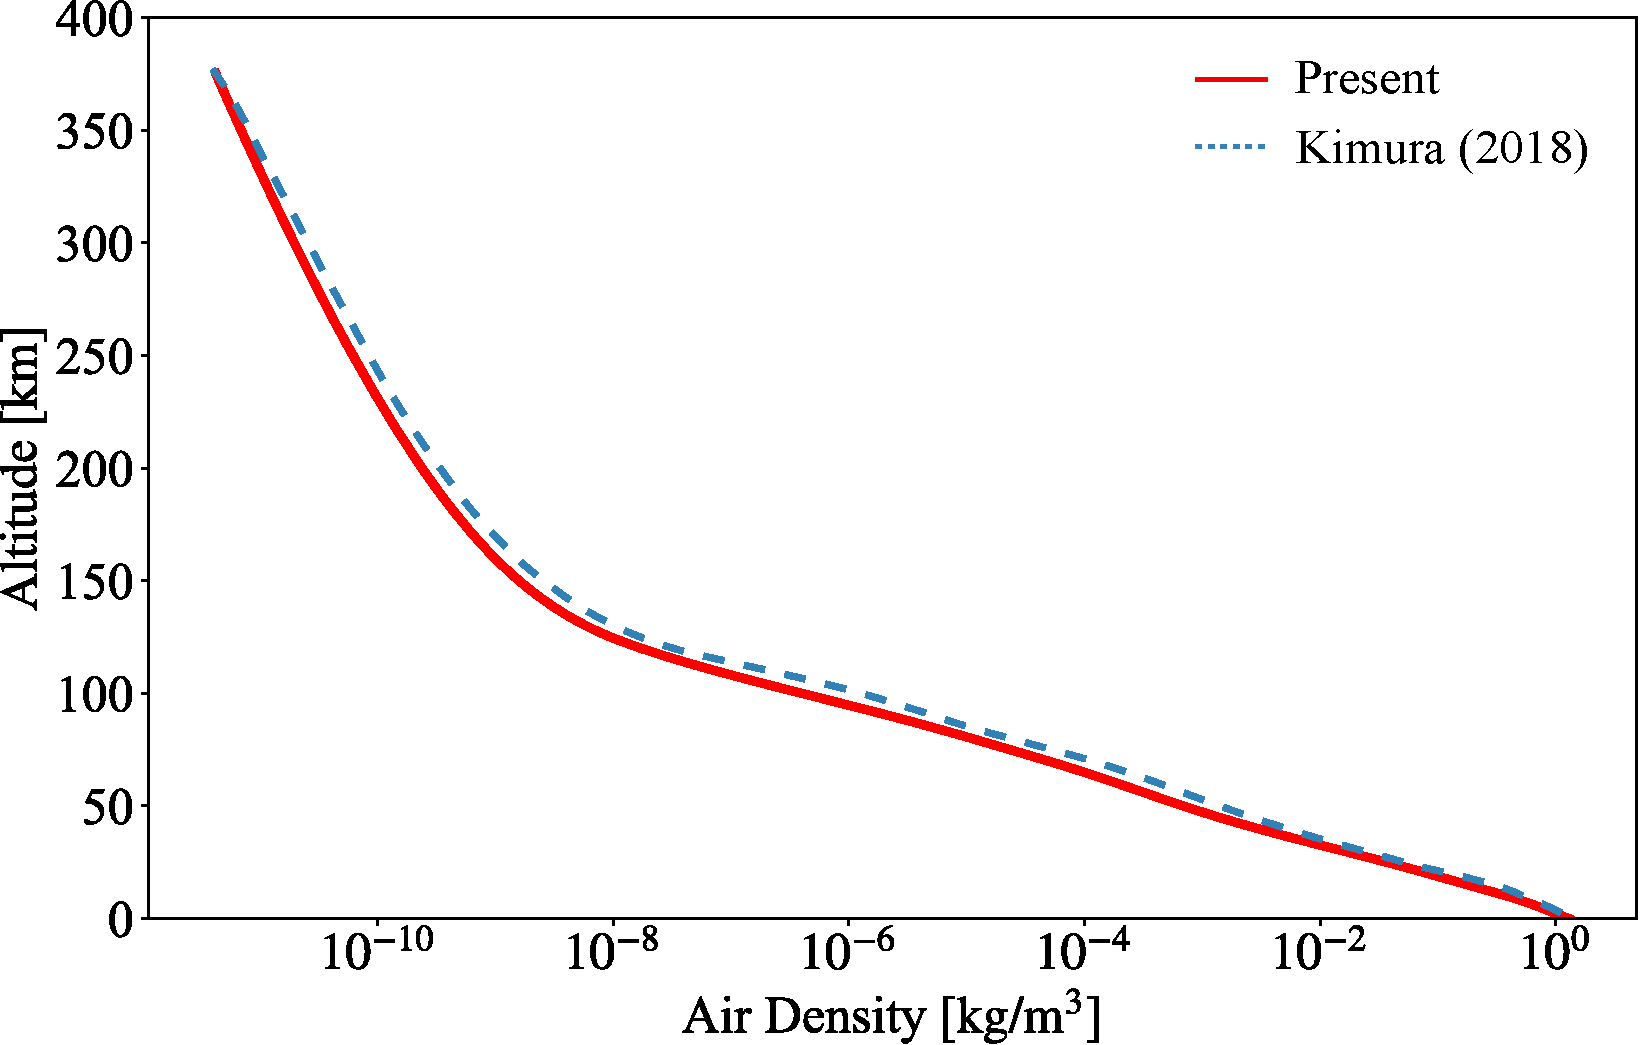
\includegraphics[width=10cm]{fig/trajectory/rho.pdf}
    \caption{大気モデルにより得られた大気密度.}
    \label{fig:trajectory-rho}
\end{figure}

次に,大気モデルにより得られた大気温度を図~\ref{fig:trajectory-temp}に示す.
高度150~km以上の高高度において先行研究との差異が生じている.
この差異は座標の差異によるものだと考えられる.
先行研究では流星源の移動に伴って座標を更新しているが,本研究では放出される方向が不明だったため初期座標で固定している.
この差異によって高高度での大気温度に差異が生じていると考えられる.
大気温度はアブレーションに影響するため,大気密度が低く対流加熱が起こりにくい高高度ではこの差異の影響はほとんどないと考えられる.
また,高度100~km以下の高度においても差異が生じているが,こちらも高高度での差異と同様に座標の差異によるものだと考えられる.
\begin{figure}[p]
    \centering
    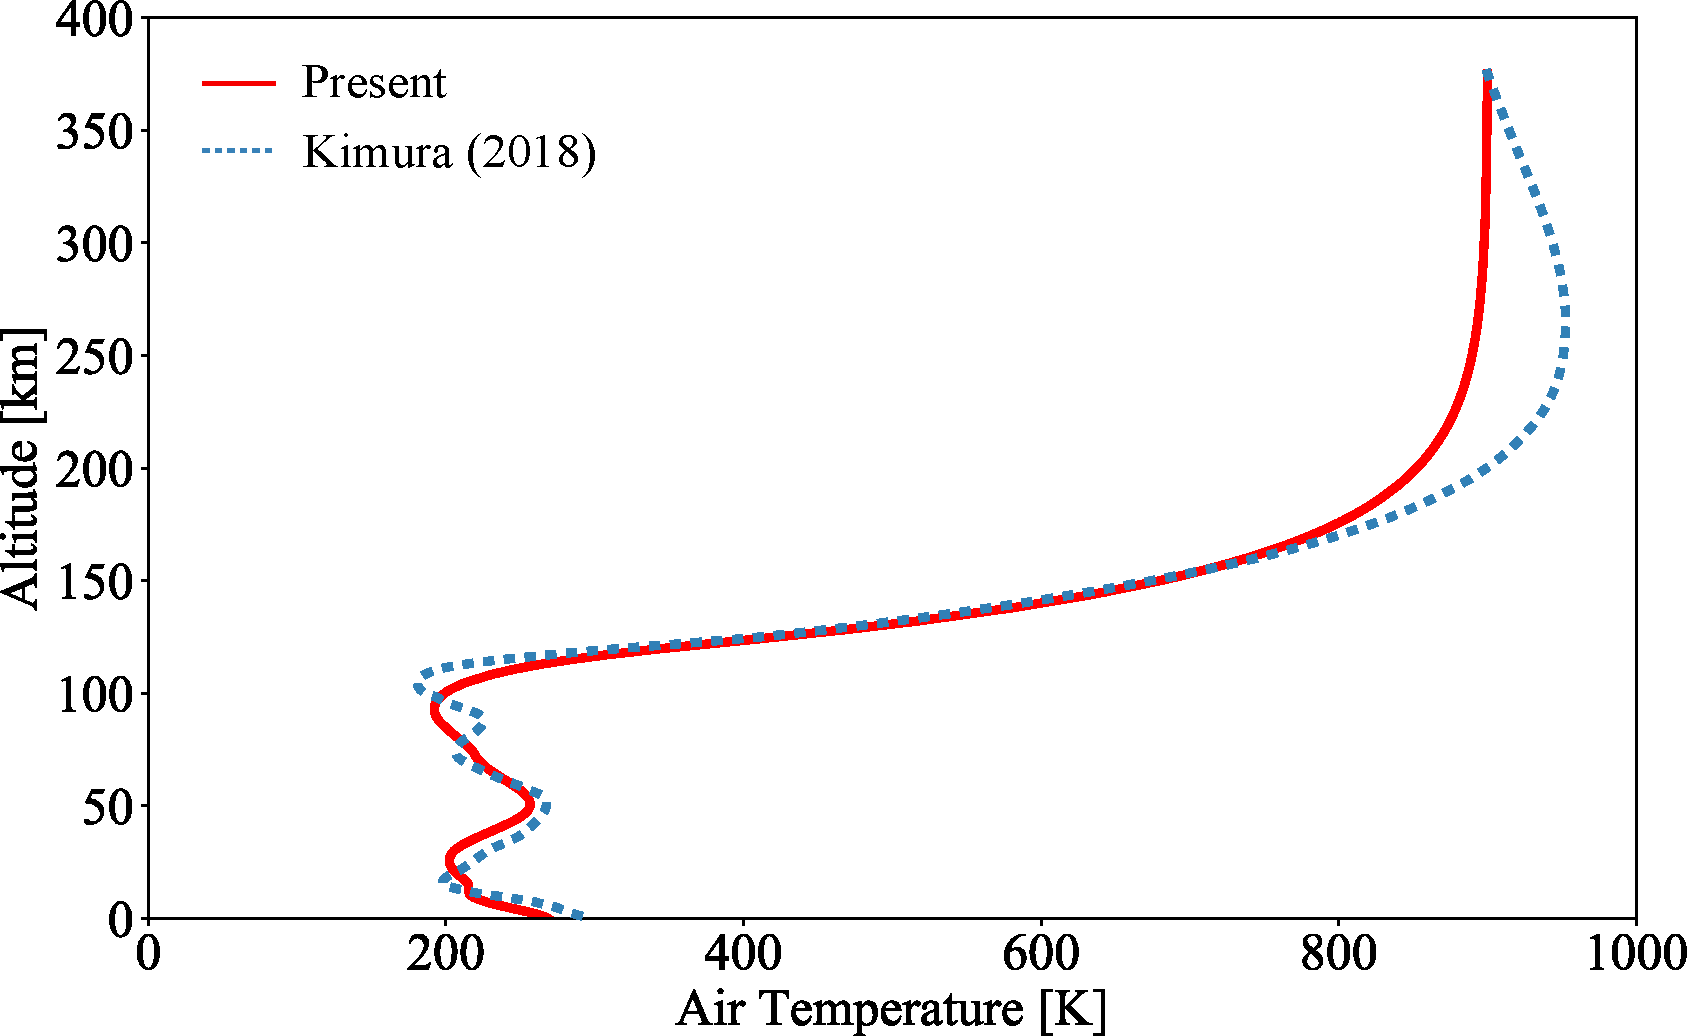
\includegraphics[width=10cm]{fig/trajectory/temp.pdf}
    \caption{大気モデルにより得られた大気温度.}
    \label{fig:trajectory-temp}
\end{figure}

\subsection{粘性係数のモデルによる違い}
木村による先行研究では粘性係数の見積もりに以下に示すSutherlandの式~\cite{sutherland1893lii}を用いている.
\begin{equation}
    \label{eq:sutherland}
    \mu = \mu_\mathrm{ref}\left(\dfrac{T}{T_\mathrm{ref}}\right)^{3/2}\dfrac{T_\mathrm{ref} + S}{T + S}.
\end{equation}
ここで,$\mu_\mathrm{ref}$,$T_\mathrm{ref}$はそれぞれ地球表面での粘性係数と温度であり,$S$はSutherland定数である.
空気における各係数は$\mu_\mathrm{ref} = \SI{1.7894e-5}{Pa.s}$,
$T_\mathrm{ref} = \SI{288.15}{K}$,
$S = \SI{110.4}{K}$とした~\cite{usstandard1976u}.

空気に対する粘性係数の見積もりにはSutherlandの式以外に知られているものがあり,代表的なものとしては以下に示すMaxwellとRayleighによるべき乗則 (Power law) が知られている.
\begin{equation}
    \mu = \mu_\mathrm{ref}\left(\dfrac{T}{T_\mathrm{ref}}\right)^{2/3}.
\end{equation}
ここで,$\mu_\mathrm{ref} = \SI{1.716e-5}{Pa.s}$, $T_\mathrm{ref} = \SI{273.0}{K}$である.

ここでは,粘性係数のモデルがどのように影響するかを先に述べた2つのモデルを比較することで検証する.
図~\ref{fig:trajectory-viscosity}にSutherlandの式とべき乗則による粘性係数分布を示す.
Sutherlandの式による見積もりの方がべき乗則による見積もりよりも変化の幅が広く,どちらのモデルも大気温度を唯一の従属変数としているため,
Sutherlandの式の方が温度変化により敏感に反応する.
しかし,大気温度と同様に差異が高高度で生じているためこの差異は無視できるとして,
先行研究で用いられているSutherlandの式を本研究でも用いることとした.
\begin{figure}[p]
    \centering
    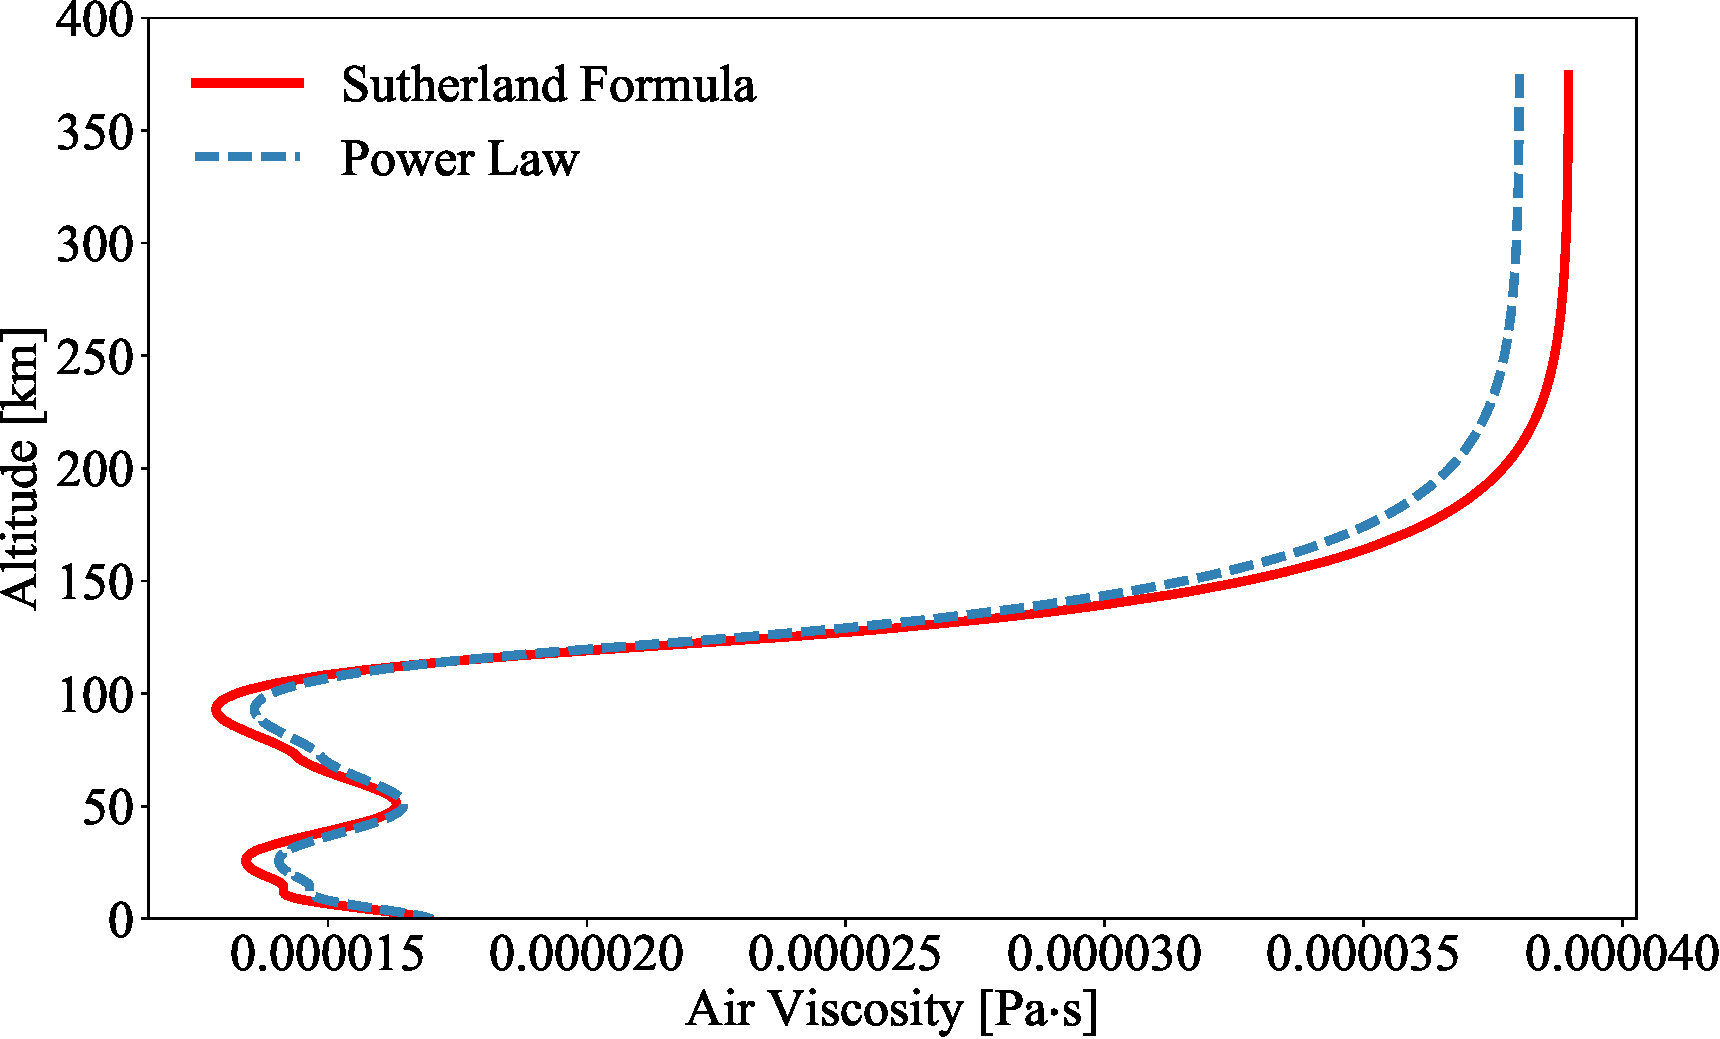
\includegraphics[width=10cm]{fig/trajectory/viscosity.pdf}
    \caption{Sutherlandの式とべき乗則による粘性係数分布.}
    \label{fig:trajectory-viscosity}
\end{figure}

\section{速度変化と質量変化の軌道計算結果}
軌道計算により得られた流星源の速度変化を図~\ref{fig:trajectory-velo}に示す.
木村による先行研究と良好に一致しており,大気密度の差異がほとんど影響を与えていない.
高度約100~km以上の高高度では大気密度が低いため動圧抵抗が小さく,従ってほとんど重力ポテンシャルによる等加速度運動で加速していることが確認される.
7,600~m/sほどまで加速した後,急に動圧抵抗を受けて数10~kmの降下で約2,500~m/sまで減速している.

\begin{figure}[p]
    \centering
    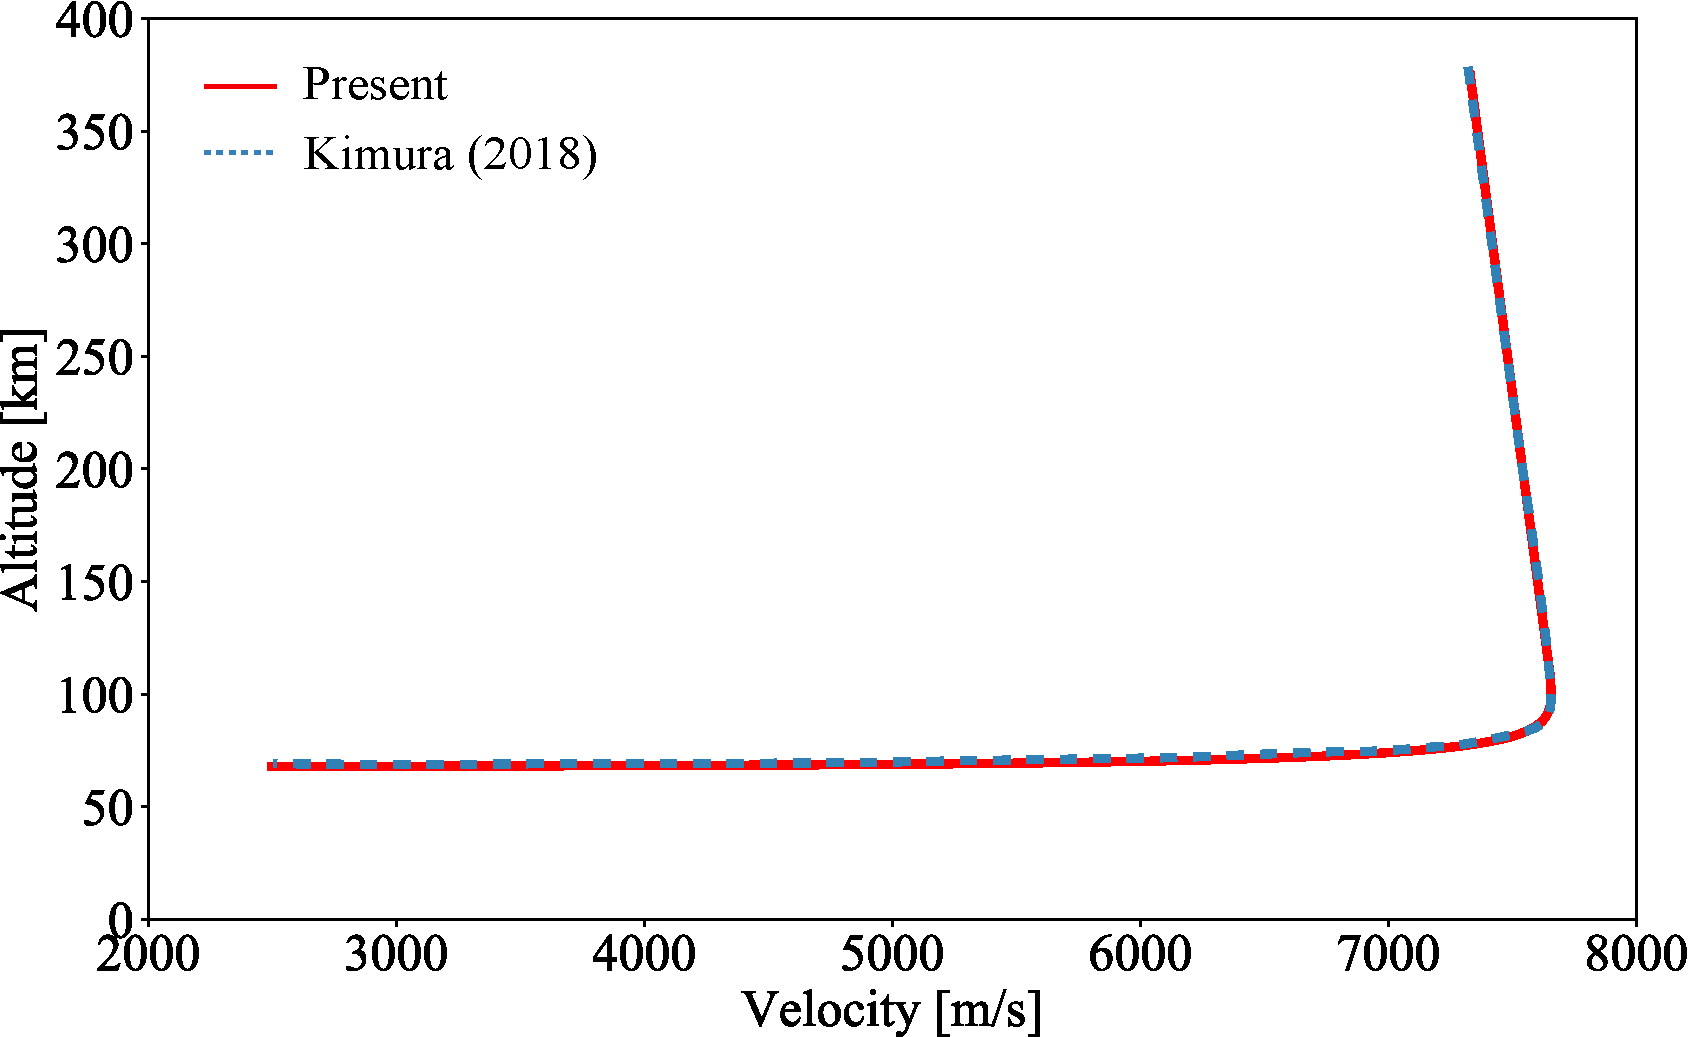
\includegraphics[width=10cm]{fig/trajectory/velo.pdf}
    \caption{軌道計算によって得られた流星源の速度変化.}
    \label{fig:trajectory-velo}
\end{figure}

また,軌道計算により得られた流星源の質量変化を図~\ref{fig:trajectory-mass}に示す.
こちらも速度変化と同様に先行研究と良好な一致を示した.
このことから大気モデルによる大気温度の差異はほとんど質量変化に影響を与えなかったと考えられる.
アブレーションによる質量減少が再現されており,高度150~km以下において空力加熱により急激に質量が減少している.

\begin{figure}[p]
    \centering
    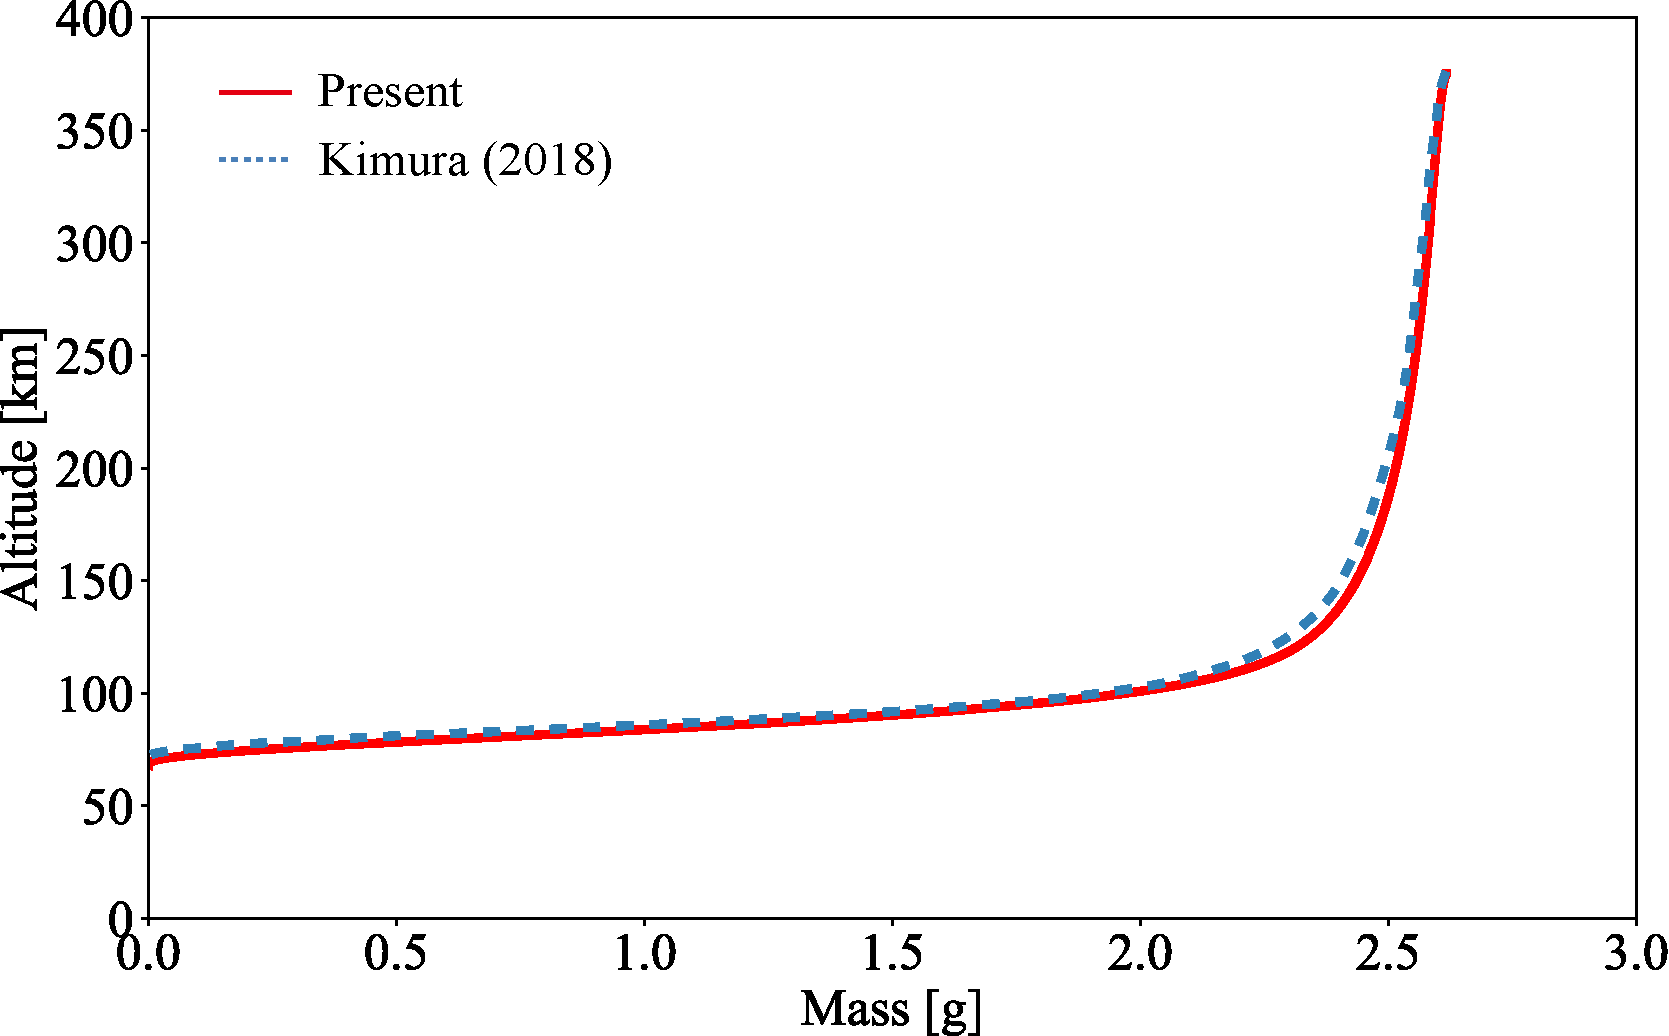
\includegraphics[width=10cm]{fig/trajectory/mass.pdf}
    \caption{軌道計算によって得られた流星源の質量変化.}
    \label{fig:trajectory-mass}
\end{figure}

\section{その他パラメータの軌道計算結果}
流体場解析において最も影響を与えるのは大気モデルと速度・質量変化であるが,軌道計算の正確性を議論するために,その他のパラメータについても先行研究と比較する.

流星源のMach数変化を図~\ref{fig:trajectory-mach}に示す.高度約200--350~kmと約70--120~kmにおいて差異が確認できる.Mach数は速度と音速の比であり,図~\ref{fig:trajectory-velo}に示すように速度については良好な一致を示したため,これは音速の差異によるものであると分かる.本研究では,音速$a$を以下のように定義している.
\begin{equation}
    a = \sqrt{\gamma RT}
\end{equation}
ただし,$R$は一般気体定数である.本研究及び木村の先行研究において比熱比$\gamma$は一定という仮定を行っているため,温度が差異に影響している.図~\ref{fig:trajectory-temp}と比較すると差異が生じる高度が概ね一致しており,温度差異がMach数に影響を与えたと考えられる.
\begin{figure}[p]
    \centering
    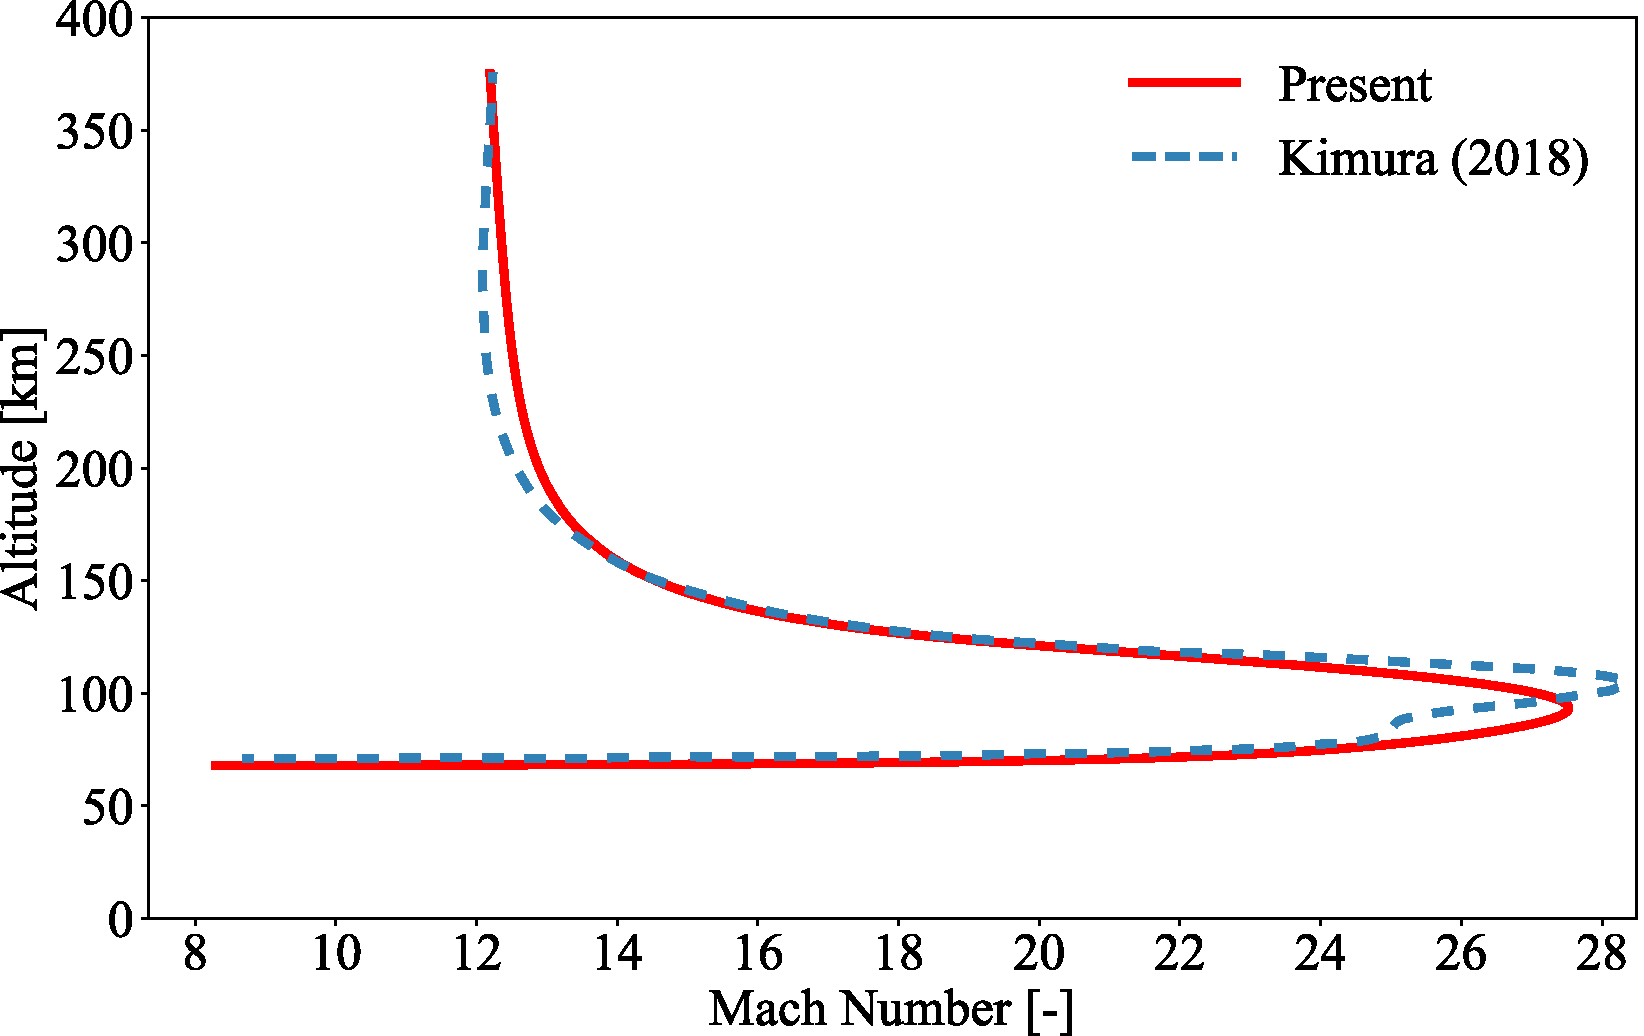
\includegraphics[width=10cm]{fig/trajectory/mach.pdf}
    \caption{軌道計算によって得られた流星源のMach数変化.}
    \label{fig:trajectory-mach}
\end{figure}

流星源のReynolds数変化を図~\ref{fig:trajectory-re}に示す.こちらもMach数同様に差異が生じているが,流星源が放たれる高度375~kmですでに差異が生じている.
この差異は粘性係数の違いによるものであると考えられる.
木村~\cite{kimura2018master}によると粘性係数をSutherlandの式で求めているが,
論文に記載のプログラムを見ると式が間違っており,
粘性係数の高度変化が本研究のものと全く異なる分布を示している.
この粘性係数の違いがReynolds数分布に影響を与えたと考えられる.
\begin{figure}[p]
    \centering
    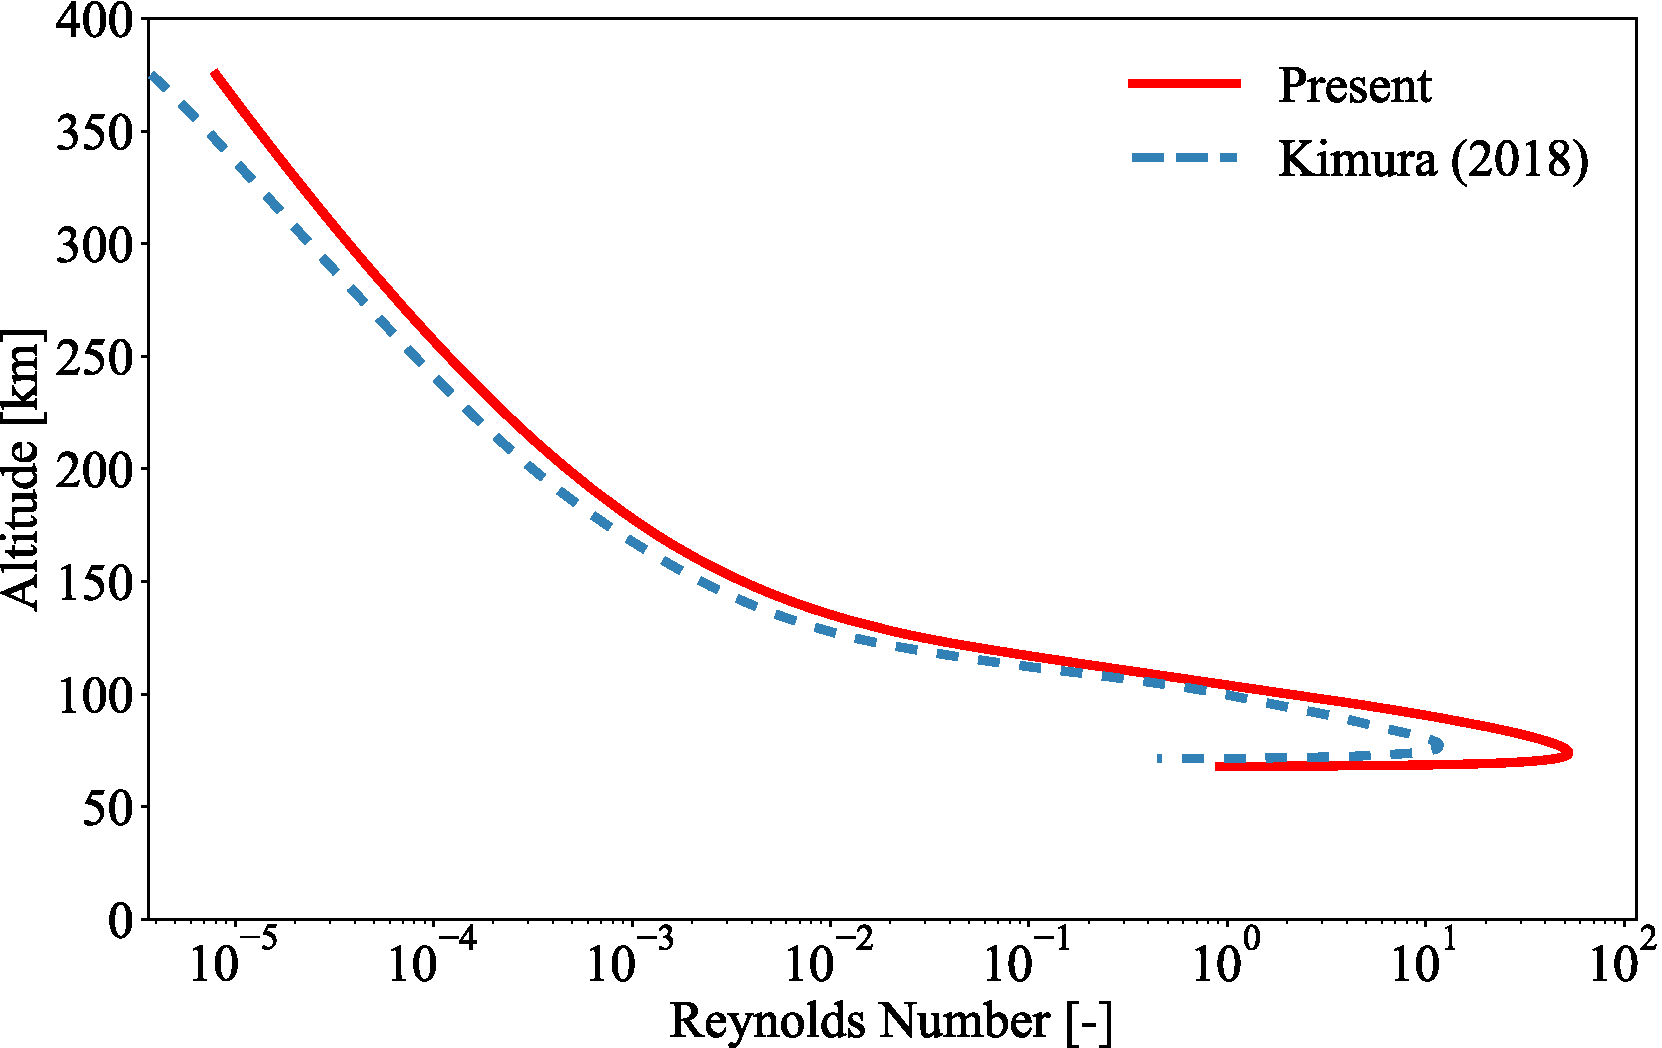
\includegraphics[width=10cm]{fig/trajectory/re.pdf}
    \caption{軌道計算によって得られた流星源のReynolds数変化.}
    \label{fig:trajectory-re}
\end{figure}

流星源のKnudsen数変化を図~\ref{fig:trajectory-kn}に示す.
Knudsen数はMach数に比例し,Reynolds数に反比例する関係にある.
従って図~\ref{fig:trajectory-re}に示したReynolds数の違いが影響し,
分布が一致していないと考えられる.
また,高度73~km地点において最小値を取っており,流星源の軌道上において最も連続流に近い高度となっている.
本研究では,この地点についての流体場解析を行い,第\ref{chap:min-knud}章でその結果を議論する.
\begin{figure}[p]
    \centering
    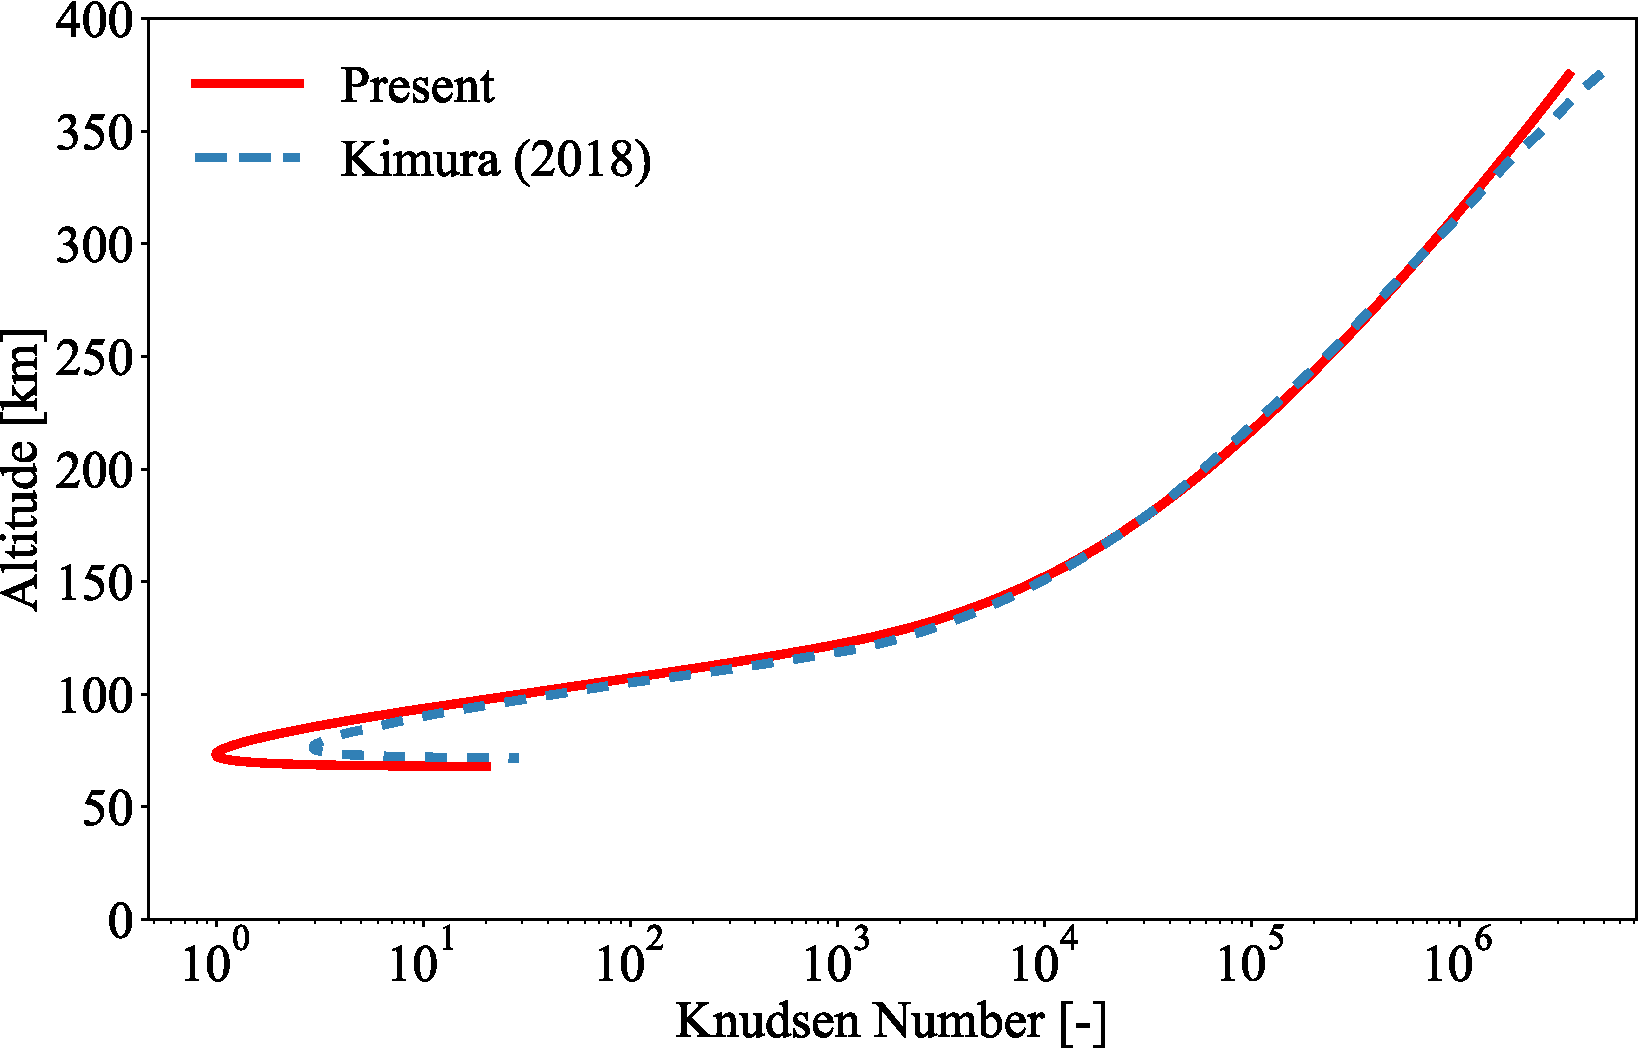
\includegraphics[width=10cm]{fig/trajectory/kn.pdf}
    \caption{軌道計算によって得られた流星源のKnudsen数変化.}
    \label{fig:trajectory-kn}
\end{figure}

流星源の抗力係数変化を図~\ref{fig:trajectory-Cd}に示す.
抗力係数はMach数・Reynolds数・大気温度の関数として求めているため,
これらのパラメータが抗力係数の差異を生じさせている.
また,抗力係数の差異は初期高度375~kmから生じているため,
粘性係数の違いによるReynolds数の差異が最も影響している.
\begin{figure}[p]
    \centering
    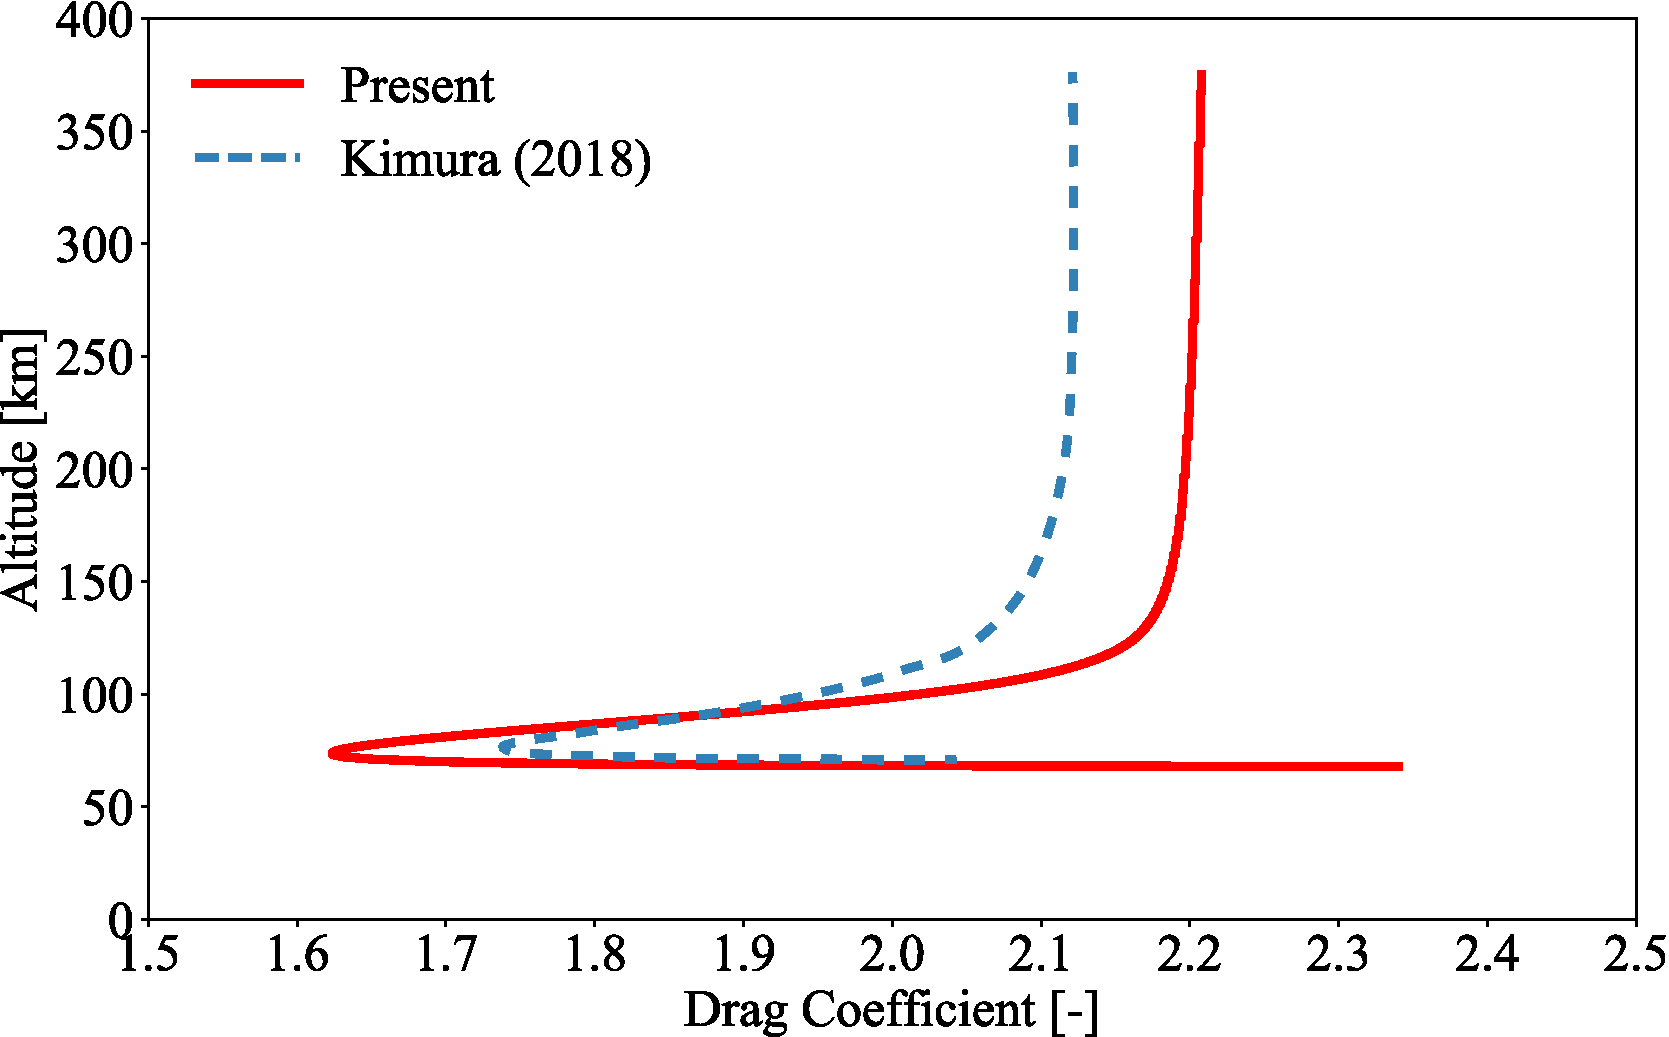
\includegraphics[width=10cm]{fig/trajectory/Cd.pdf}
    \caption{軌道計算によって得られた流星源の抗力係数変化.}
    \label{fig:trajectory-Cd}
\end{figure}

流星源が受ける熱流束変化を図~\ref{fig:trajectory-heat}に示す.
熱流束の見積もりに用いているDKRモデルは流星源半径・速度・大気密度の関数であり,それらの差異が熱流束に差異を与えているものの,概ね良好な一致を示している.
\begin{figure}[p]
    \centering
    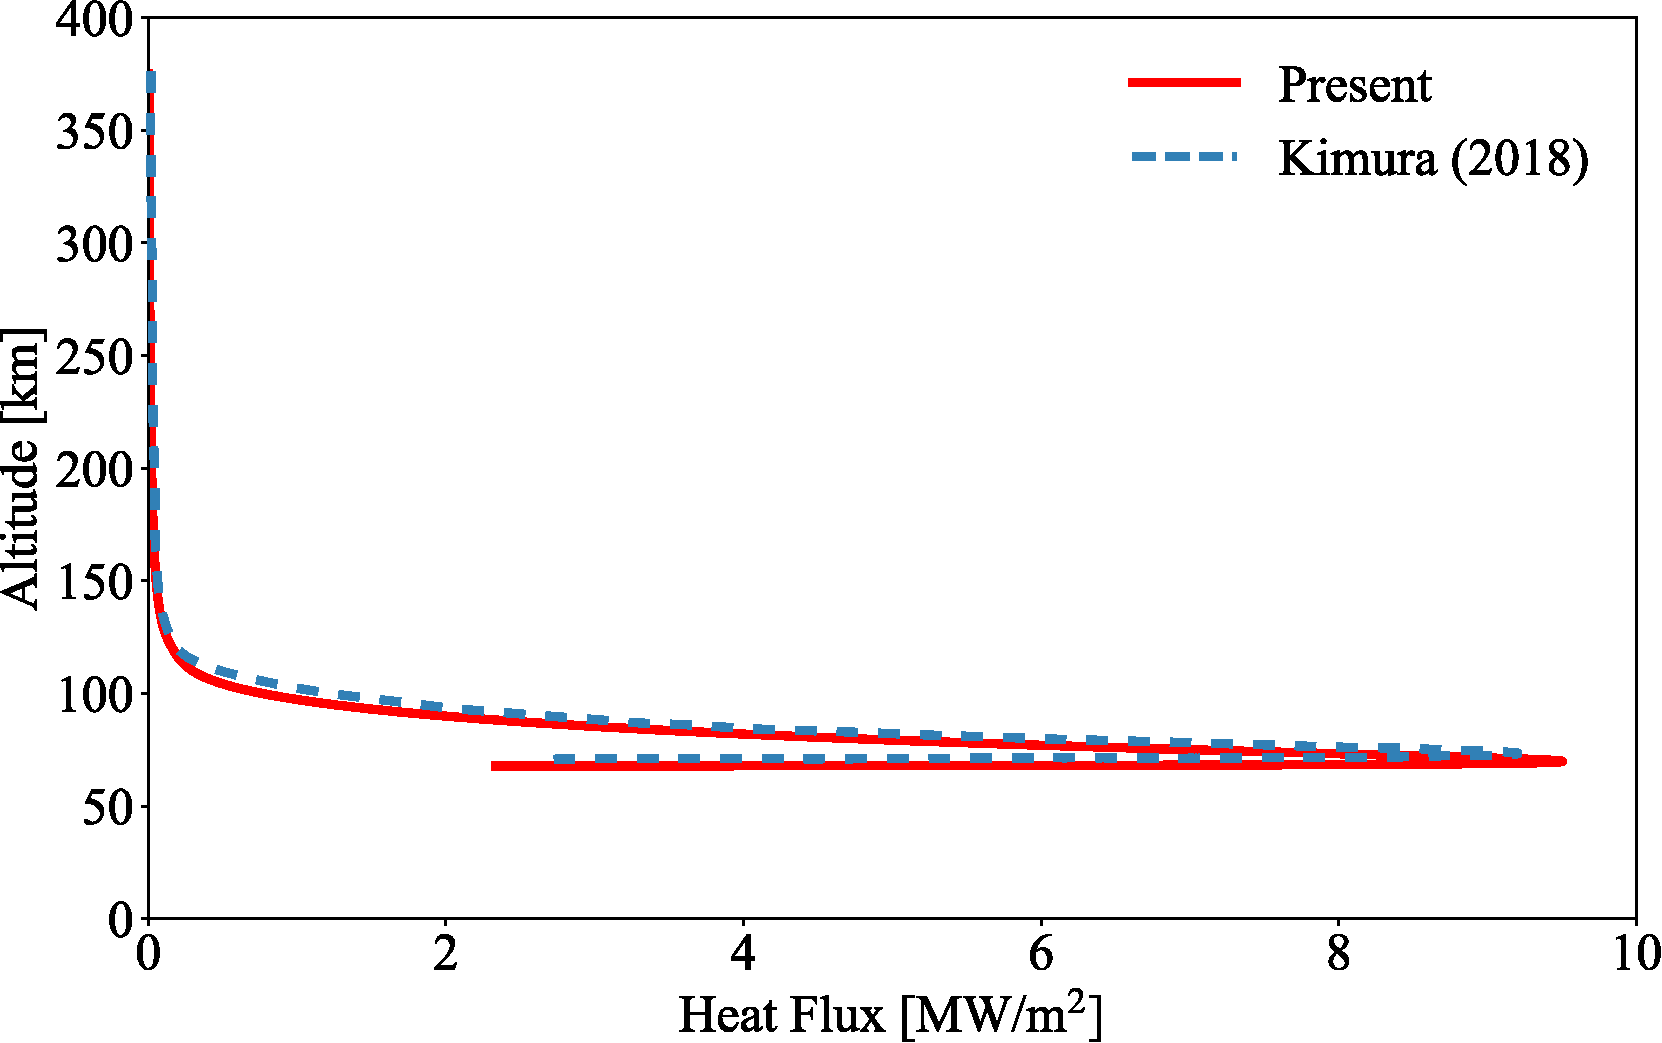
\includegraphics[width=10cm]{fig/trajectory/heat.pdf}
    \caption{軌道計算によって得られた流星源が受ける熱流束変化.}
    \label{fig:trajectory-heat}
\end{figure}

最後に,流星源の熱伝達係数変化を図~\ref{fig:trajectory-Ch}に示す.
抗力係数とは異なり,概ね良好に一致したが,初期高度375~kmで差異が見られる.
熱伝達係数はMach数と熱流束の関数となっており,
粘性係数が異なるために生じる初期高度でのMach数の差異が影響を及ぼしていると考えられる.
\begin{figure}[p]
    \centering
    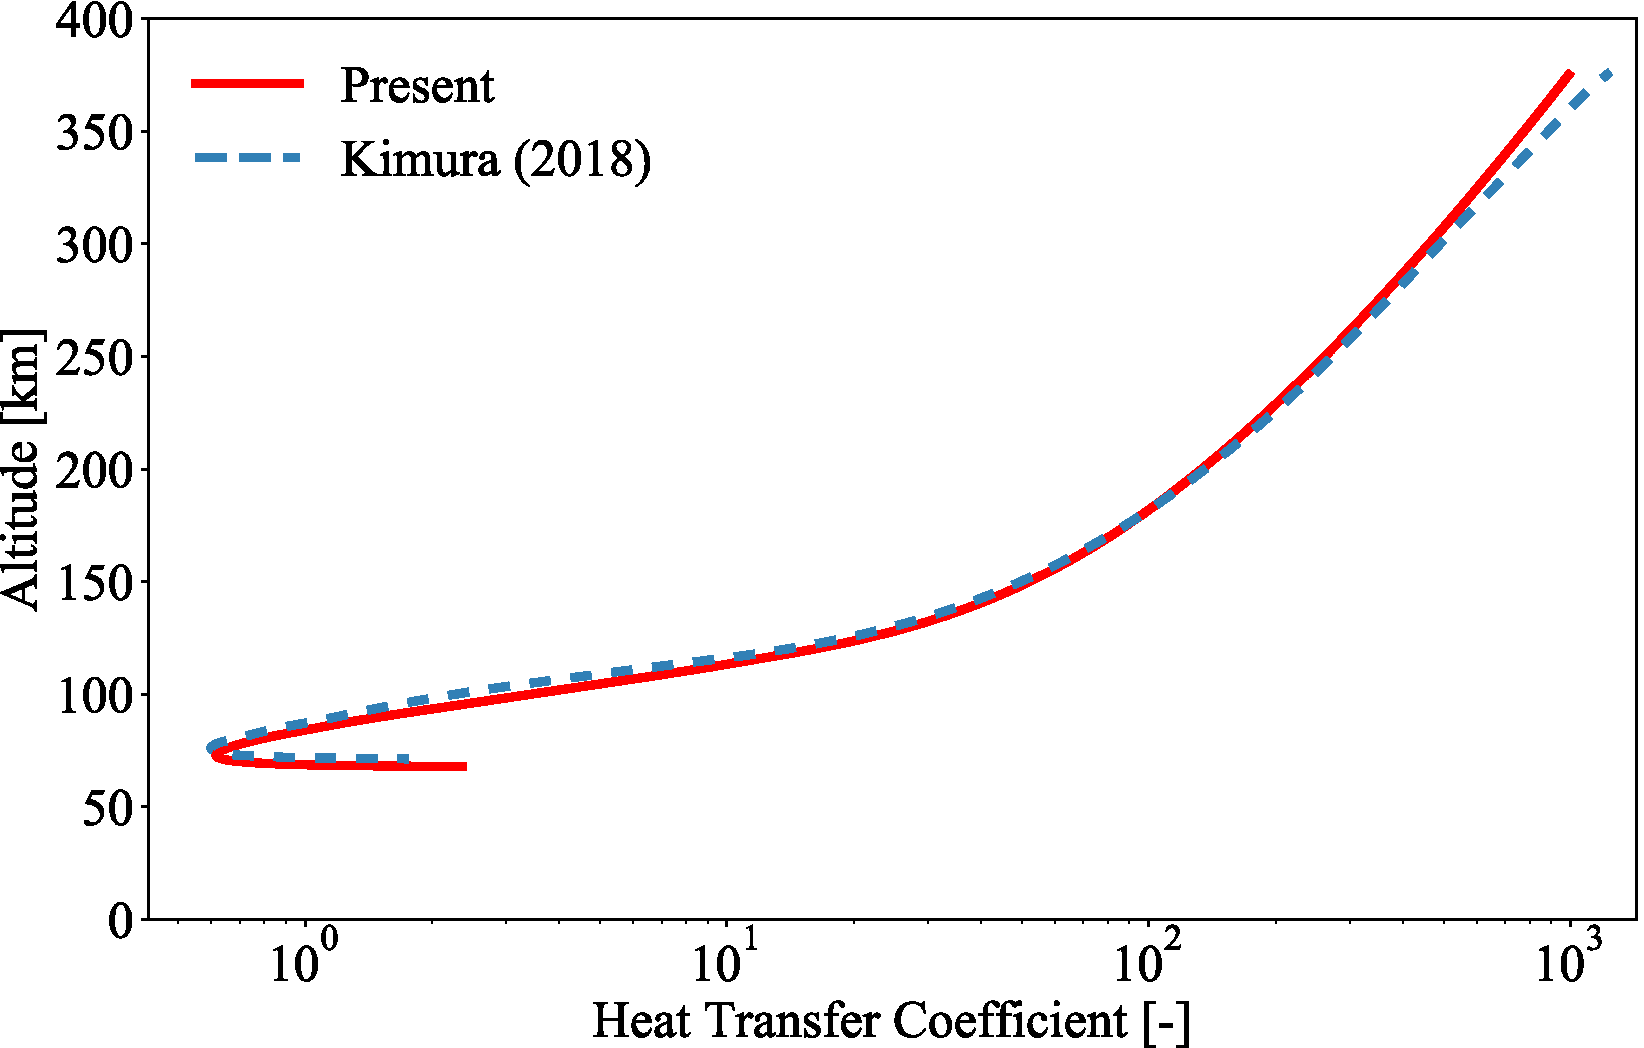
\includegraphics[width=10cm]{fig/trajectory/Ch.pdf}
    \caption{軌道計算によって得られた流星源の熱伝達係数変化.}
    \label{fig:trajectory-Ch}
\end{figure}

%\section{本章のまとめ}
%本章では,流星源の軌道計算結果を述べた.
%まず,木村~\cite{kimura2018ukaren}と同様に設定した初期条件を示した.
%次に大気モデルの結果を示した.
%大気密度は良好な一致を示したが,
%大気温度に差異が現れた.
%この差異は,座標を更新せずに初期座標で固定しているためであると考えられる.
%次に,粘性係数のSutherlandの式とべき乗則モデルの違いを調べた.
%両者は概ね一致したため,Sutherlandの式を採用した.
%
%流星源の速度と質量変化の分布を示した.
%先行研究と本研究で得られた結果は良好な一致を示した.
%また,その他の無次元量やパラメータについては大気モデルの温度差異によって差異を生じていることが分かった.
%特に粘性係数については,先行研究で用いられた式が間違っており,従ってReynolds数やKnudsen数,抗力係数にその違いが顕著に現れた.
%
%これらの差異は無視できるとは言い切れない.
%しかし,速度変化と質量変化を比較すると良好に一致し,この差異に対する感度が小さいことが分かる.
%流体場解析において重要になるのは,主流条件や流星源の大きさであり,
%大気温度・大気密度・速度変化・質量変化が概ね一致しているため,
%これらの結果は妥当であるとする.
%従って流体場解析の条件としては本章での軌道計算で得られた結果を採用する.